\subsection{The transactions as a graph}
\label{sec:expl:graph}

Every on-chain fill is a meeting between a wallet and a market, so the transactions table
of \cref{sec:data:sources} is, read as a whole, a bipartite graph: wallets on one side,
markets on the other, one edge for every pair that traded at least once, weighted by the
number of fill legs between them.  The graph is the input of the models of
\cref{ch:graph}; this section describes it as an object, before any model reads it.  The description is purely descriptive, uses no label and no
model, and is therefore computed on the whole window of twenty-one days, the locked test
days included.  The numbers come from the exact graph (every fill leg of the window,
\cref{app:reproduction}); the maps come from a two-dimensional layout described in
\cref{sec:expl:graph:map}.

\begin{figure}[p]
\centering
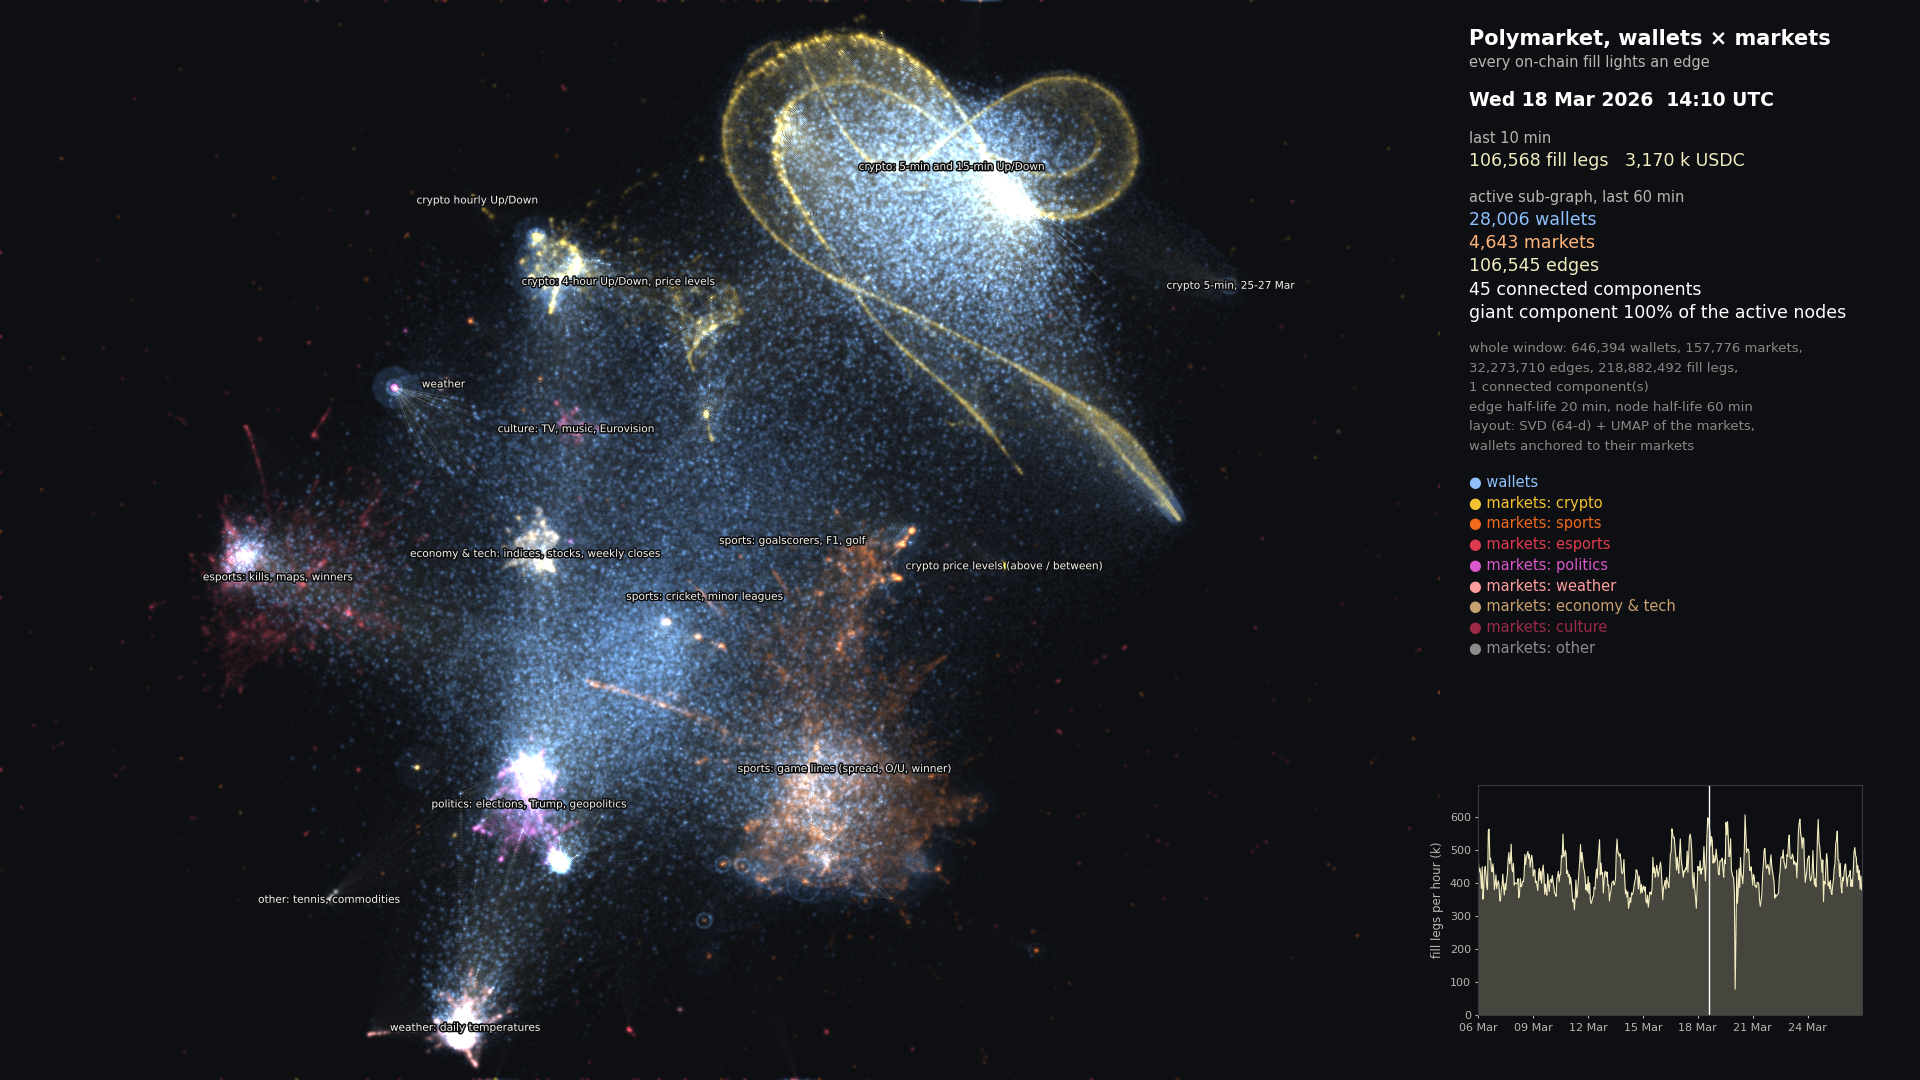
\includegraphics[width=\textwidth]{figures/graph/graph_frame_18mar.png}
\caption{One frame of the animation of the transaction graph: Wednesday 18 March 2026,
14:10 UTC.  Every fill of the last minutes lights the edge between a wallet and a market
and fades with a half-life of twenty minutes; wallets are blue, markets are coloured by
category (crypto yellow, sports orange, esports red, politics violet, weather pink,
economy and tech brown, culture dark red); the largest islands of the map carry their
label.  The side panel gives the activity of the bin and the active sub-graph of the last
hour.  The ribbon at the top right is the crypto five- and fifteen-minute contracts; the
bright blobs are the markets whose public is active in those minutes.}
\label{fig:graph:frame}
\end{figure}

\subsubsection{Size, density and heavy tails}
\label{sec:expl:graph:size}

\begin{table}[t]
\centering
\caption{The wallet--market transaction graph of 6--26 March 2026.}
\label{tab:graph:stats}
\small
\begin{fittable}\begin{tabular}{ll}
\toprule
Quantity & Value \\
\midrule
fill legs (edge events) & 218{,}882{,}492 (78{,}931{,}041 taker fills) \\
wallets & 646{,}394 \\
markets & 157{,}776 \\
distinct wallet--market edges & 32{,}273{,}710 \\
bipartite density & $3.2 \times 10^{-4}$ \\
wallet degree (markets traded): median / mean / max & 4 / 49.9 / 41{,}767; 22.5\% of the wallets have degree 1 \\
market degree (wallets seen): median / mean / max & 29 / 204.6 / 16{,}816; no market below 2 \\
edge multiplicity (fills per pair): median / p99 / max & 2 / 107 / 101{,}367; 47.6\% of the edges carry one fill \\
connected components, whole window & 1 (all 804{,}170 nodes) \\
$k$-core: largest core / nodes in it / nodes with core $\ge 10$ & 685 / 8{,}428 / 339{,}471 \\
concentration & top 1\% of wallets make 77.9\% of the fill legs (Gini 0.963) \\
                & top 1\% of markets receive 16.6\% (Gini 0.836) \\
\bottomrule
\end{tabular}\end{fittable}
\end{table}

\Cref{tab:graph:stats} gives the graph in numbers and \cref{fig:graph:summary}(a) its
degree distributions.  The graph is sparse as a matrix, three edges in ten thousand
possible pairs, and dense as a social object: every market has been traded by at least two
wallets and by twenty-nine in median, and the whole graph is \emph{one} connected
component, with no isolated pair and no small island.  Its three distributions have the
heavy tails of every interaction network: the median wallet traded four markets and the
most active 41{,}767; the median market was traded by 29 wallets and the most popular by
16{,}816; the median edge carries two fills and the heaviest a hundred thousand.
Concentration is extreme on the wallet side, where one wallet in a hundred makes more
than three quarters of the fill legs, and much milder on the market side, where the top
one per cent of the markets takes one sixth of the activity: the activity is spread over
many markets but made by few hands.  The $k$-core decomposition locates those hands: a
core of 8{,}428 nodes in which every node has at least 685 neighbours inside the core, and
a third of all nodes with a coreness of at least ten.

\begin{figure}[t]
\centering
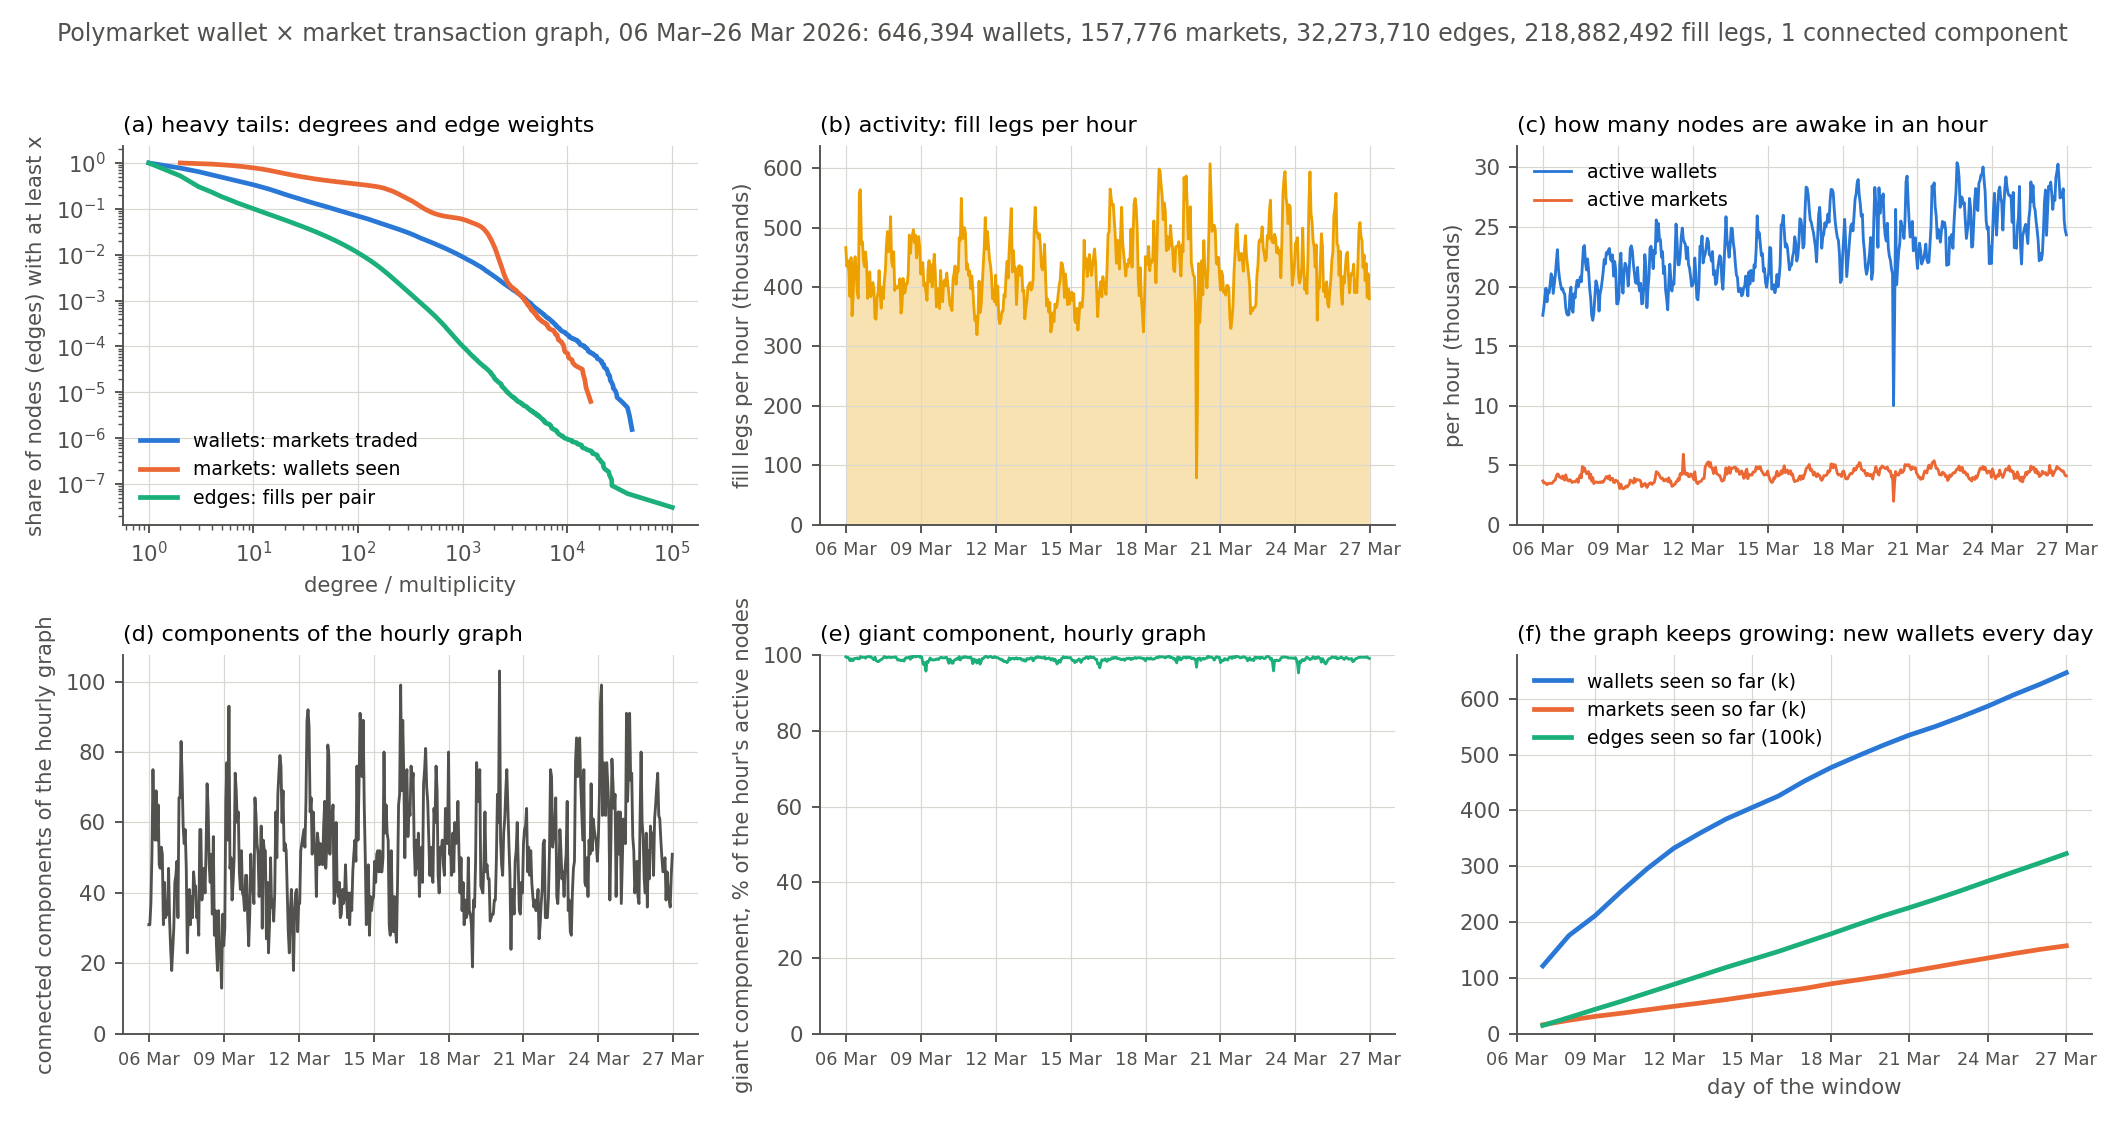
\includegraphics[width=\textwidth]{figures/graph/graph_summary.png}
\caption{The transaction graph in six panels.  (a) Complementary cumulative distributions
of the wallet degree, the market degree and the edge multiplicity (log--log).  (b) Fill
legs per hour over the window.  (c) Active wallets and active markets per hour.  (d)
Connected components of the hourly graph.  (e) Share of the hour's active nodes in its
giant component.  (f) Cumulative number of wallets, markets and edges seen since the start
of the window.}
\label{fig:graph:summary}
\end{figure}

\subsubsection{The graph in time}
\label{sec:expl:graph:time}

The hourly slices of \cref{fig:graph:summary}(b--e) show the graph as a process.  An
average hour has 434 thousand fill legs (79 thousand in the dip of 20 March, 607 thousand
at the peak), 23 thousand active wallets, rising from about 20 to about 27 thousand over
the month, and 4{,}200 active markets.  The hourly graph has 87 thousand distinct edges,
and 74\% of them are seen for the first time in the window: most of what happens in an
hour is a wallet trading a market it had never traded before, and 1{,}300 wallets per hour
have never been seen at all.  The hour-of-day profile in UTC is nearly flat (peak at 14 h,
trough at 4 h, ratio 1.32), the signature of a venue whose public is spread over the time
zones and whose busiest contracts, the crypto intervals, never close.  The hourly graph is
not connected, it has 51 components on average (13 to 103), but its giant component holds
99\% of the hour's active nodes and never less than 95\%: the small components are a few
wallets on a few markets that nobody else touched that hour.  Cumulatively
(\cref{fig:graph:summary}(f)) the graph never stops growing: 56 components after the first
day, 9 after four, 2 after six, one from the eleventh day on, and a straight line of new
wallets, new markets and new edges to the end of the window.  A model that keeps a state
per wallet, as the graph models of \cref{ch:graph} do, therefore meets at every hour a
population of which a part has no history at all.

\subsubsection{A map of the graph}
\label{sec:expl:graph:map}

\begin{figure}[p]
\centering
\begin{subfigure}{0.86\textwidth}
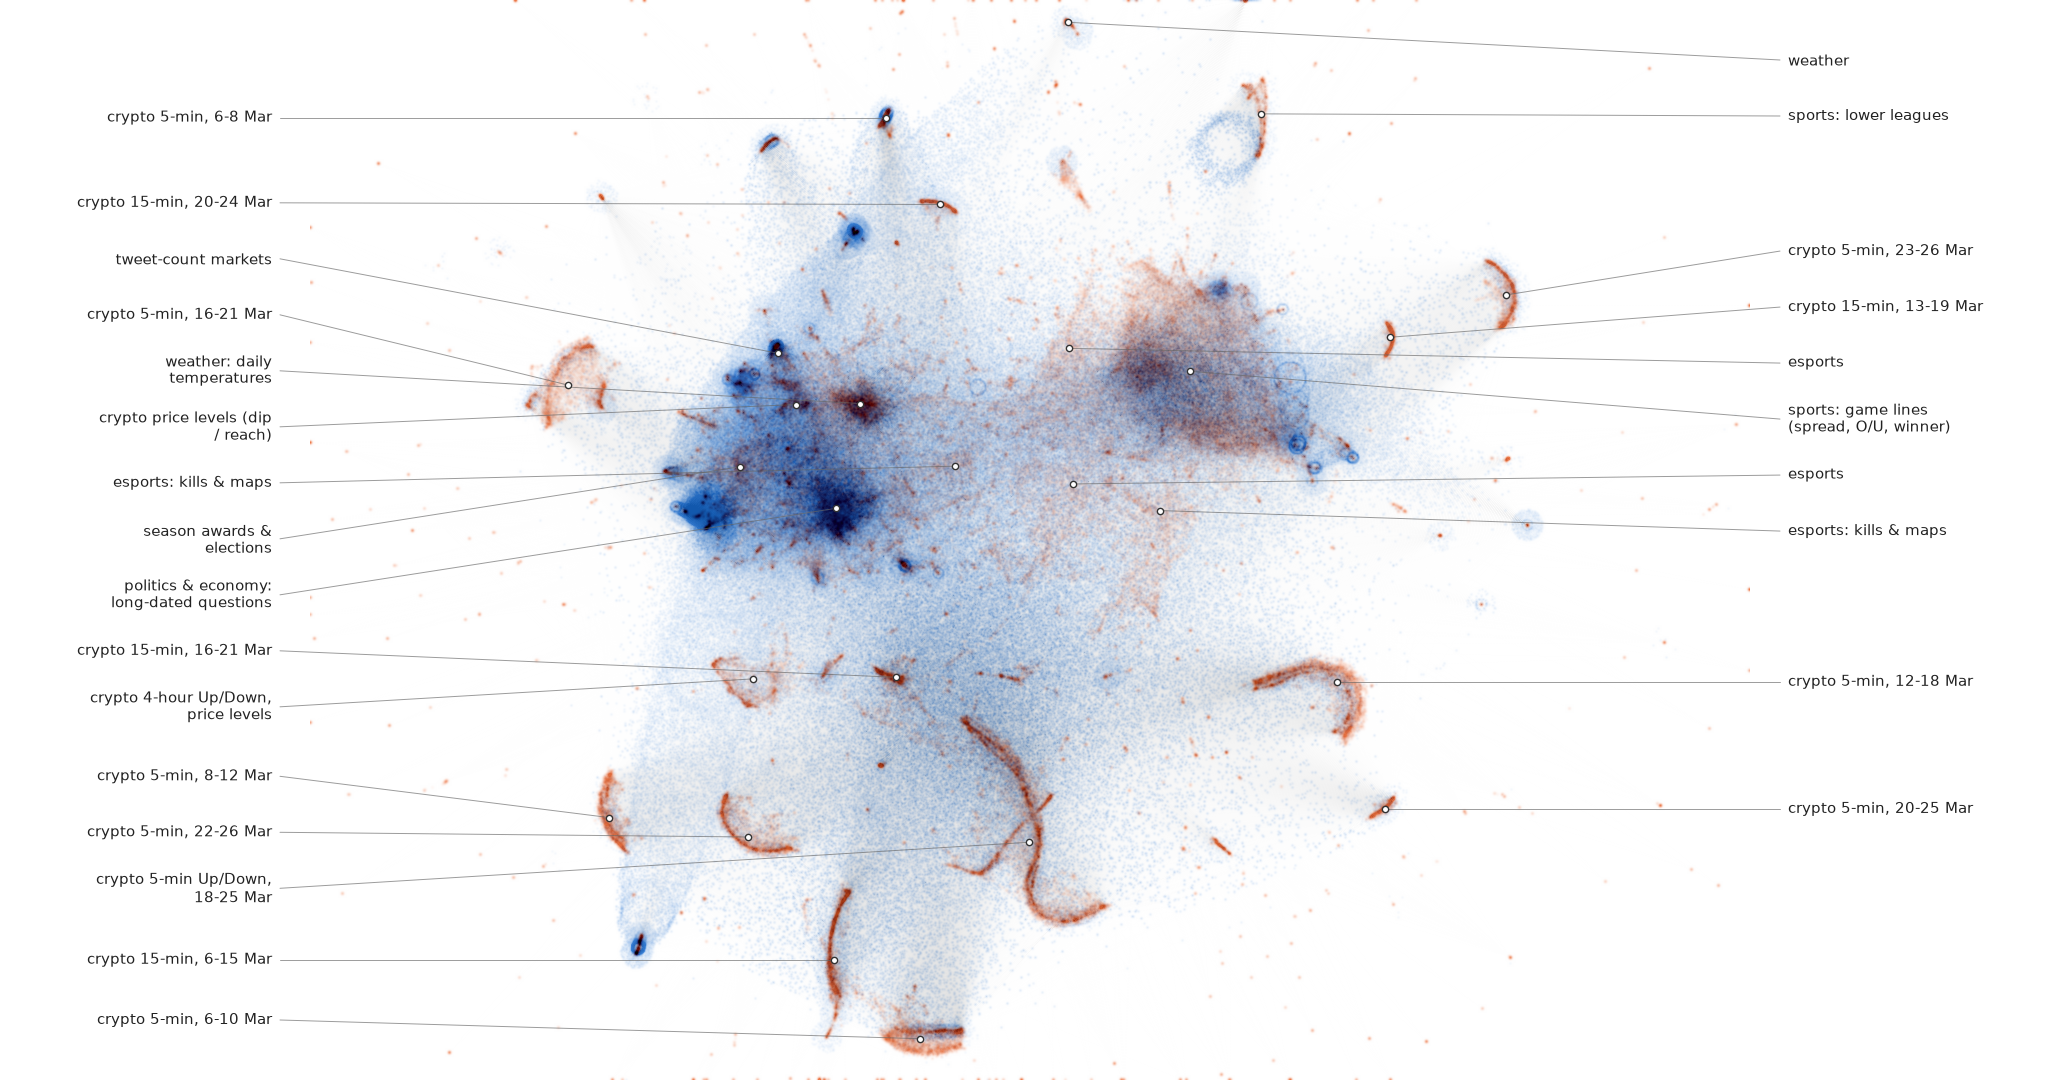
\includegraphics[width=\textwidth]{figures/graph/graph_map_similarity.png}
\caption{Markets placed by trading similarity only.}
\label{fig:graph:map:sim}
\end{subfigure}

\medskip
\begin{subfigure}{0.86\textwidth}
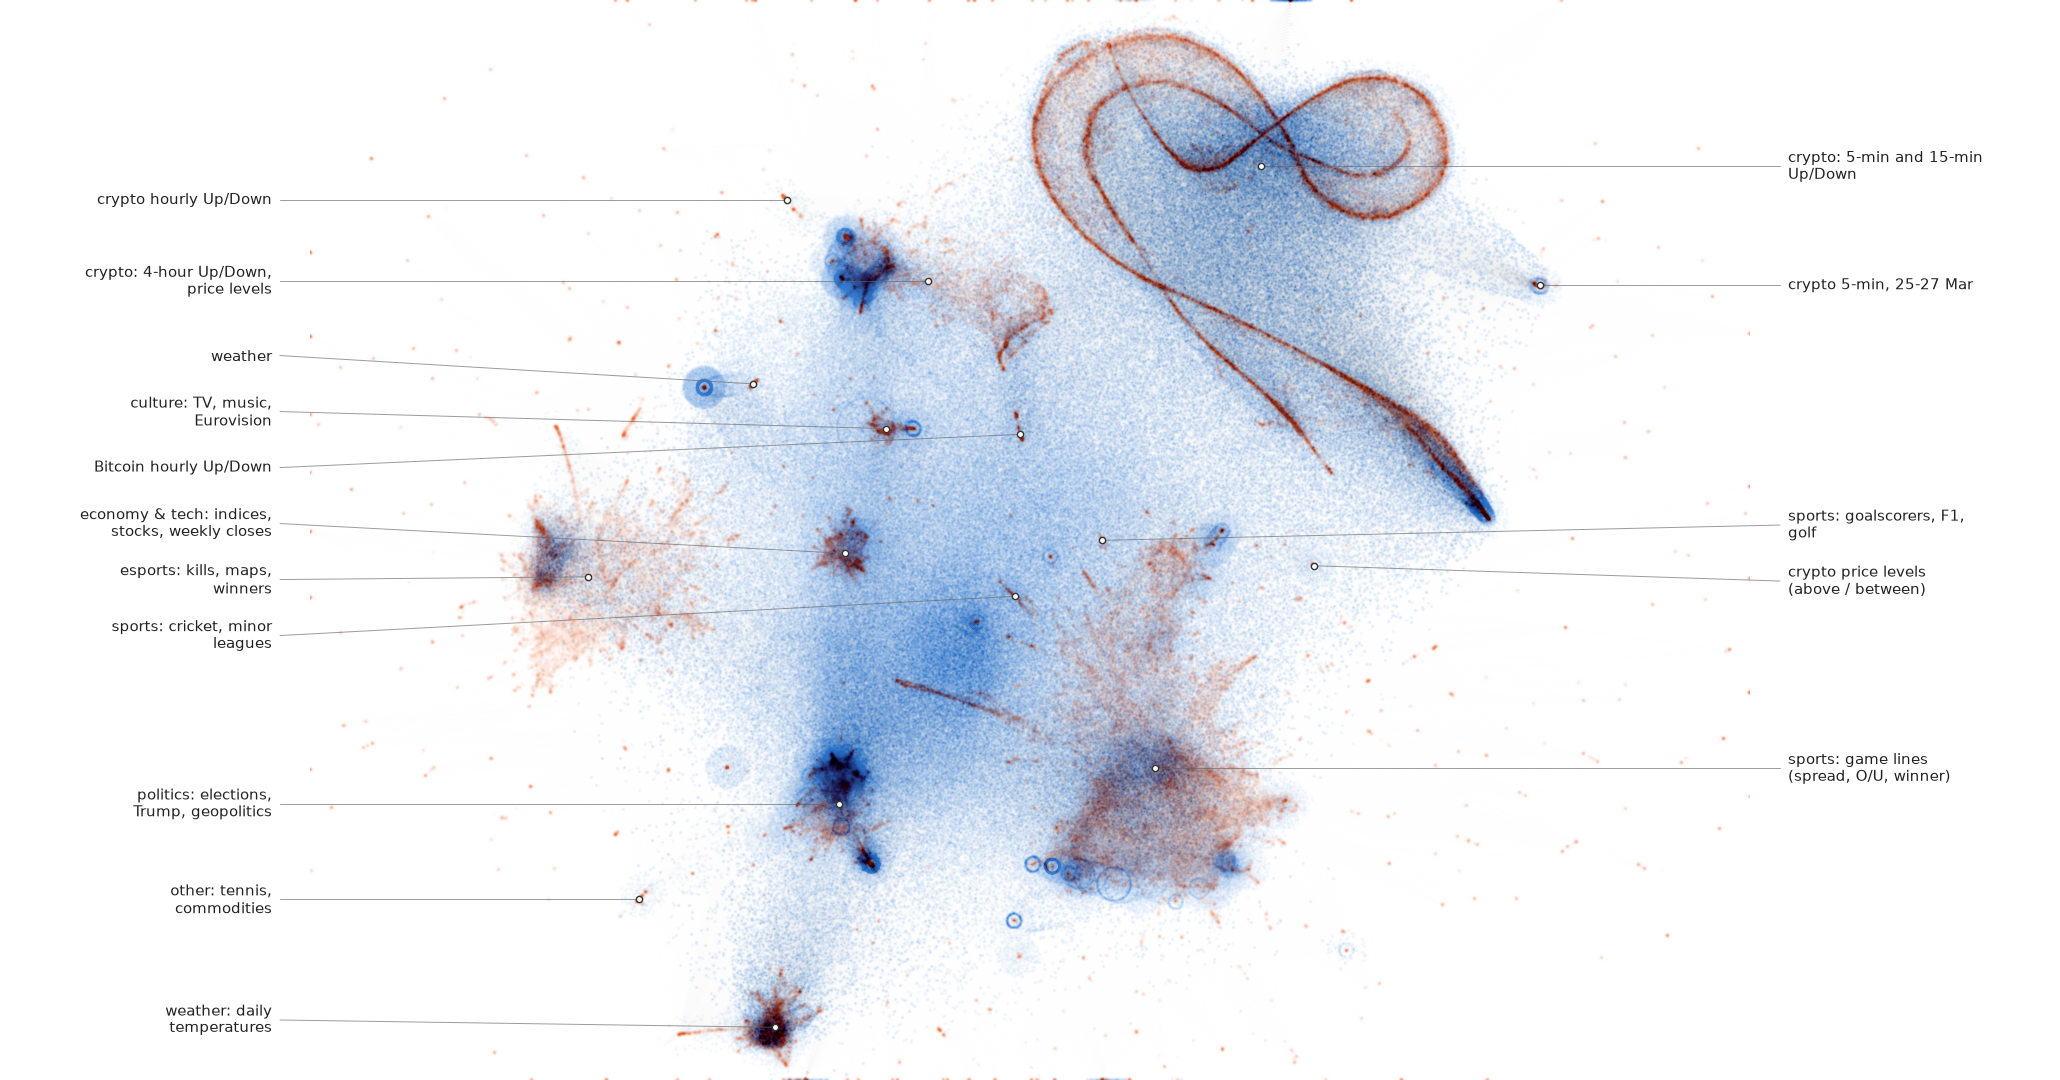
\includegraphics[width=\textwidth]{figures/graph/graph_map_category.png}
\caption{Markets placed by similarity and category.}
\label{fig:graph:map:cat}
\end{subfigure}
\caption{Two maps of the whole transaction graph (646 thousand wallets in blue, 158
thousand markets in orange, six million of the edges as faint lines).  (a) The
markets are laid out by UMAP on the trading-similarity space alone; the islands are groups
of markets traded by the same wallets, and the crypto five- and fifteen-minute contracts
form one island per few days, because the wallets that trade them on a given day are
largely the wallets of that day.  (b) The category of the market is added to the distance,
and the map separates into one region per category, with the date as the internal order
of the crypto ribbon.  Labels are the largest islands found by HDBSCAN on each map; wallets
are placed at the centroid of the markets they trade, so the dense blue regions are the
publics of the corresponding markets and the blue rings are the exclusive publics of single
markets.}
\label{fig:graph:maps}
\end{figure}

A graph of 800 thousand nodes and 32 million edges cannot be drawn by a force-directed
layout.  The maps of \cref{fig:graph:maps} use a two-step large-graph technique.  First,
the biadjacency matrix, with $\log(1 + \text{fills})$ weights, an inverse-frequency scaling
of the market columns and unit-length wallet rows, is reduced by a truncated singular value
decomposition to 64 dimensions, which gives wallets and markets a common latent space in
which two markets are close when they are traded by the same wallets.  Second, the 157{,}776
markets are mapped to the plane by UMAP \cite{mcinnes2018umap} on that space (cosine
distance, fifteen neighbours), and every wallet is placed at the fill-weighted centroid of
the markets it traded, pushed outwards in proportion to how spread those markets are, with
a deterministic halo for the wallets that traded a single market.  The second map adds to
the latent vector of every market a block that encodes its category, so that two markets of
different categories are pushed apart by a fixed amount on top of their similarity
distance.

The islands of the first map, found by HDBSCAN on the market positions (minimum size
150), are 129 and hold 79\% of the markets and 93\% of the fills; the islands of the second
map are 39 and hold 95\% of the markets.  Read with the question texts of their markets, the
islands say how Polymarket's trading is organised.  The first partition is the
\emph{category}: sports game lines (spreads, totals, winners) are the largest island of
the first map with 24{,}624 markets, and on the second map every category is a continent
of its own, sports with 48 thousand markets, crypto with 44 thousand and 148 million fill
legs, two thirds of all the activity of the venue, esports with 19 thousand, then politics,
weather, economy and culture.  Inside crypto the second partition is the \emph{contract
length and the date}: the five- and fifteen-minute Up/Down contracts live a few minutes
each, a new one opens as the previous one closes, and the wallets that trade them on a
given day form the island of that day, so that the first map has one crypto island per two
to five days and the second map a single ribbon whose internal order is still the date.
The longer crypto contracts (hourly, four-hour, price levels) are separate islands in both
maps, as are the daily temperature markets, the tweet-count markets and the long-dated
political questions.  The organisation of the trading is thus the organisation of
\cref{sec:expl:templates} seen from the wallets' side: who trades what is decided first by
the category and then by the type of contract, and the families of markets defined by how
they trade (\cref{sec:structure:markets}) are a third partition that cuts across both.

\subsubsection{Large taker orders}
\label{sec:expl:graph:bursts}

The animation from which \cref{fig:graph:frame} is taken shows, now and then, a blue disc
lighting up at once: several hundred wallets that traded nothing else in the whole window,
all filled within the same minutes.  The disc shape is an artefact of the layout, which
draws single-market wallets in a halo around their market; the burst itself is the
footprint of one very large taker order.  An order that crosses the book is filled against
the resting orders on the other side, and when the resting side is made of many small
orders from many wallets, one transaction creates hundreds of edges in one block.  The
largest such bursts (575 one-market wallets on a basketball spread in ten minutes on
20 March; 466 on a basketball total; 227 on a recession question) have exactly this
anatomy: all the wallets are \emph{makers}, filled by one or a few taker transactions that
each consume about a hundred resting orders from a hundred distinct wallets, at the same
prices and with a handful of distinct sizes, and most of those wallets have exactly one
fill in the whole month.  Such transactions are marginal in volume: those with at least
fifty maker legs of which four fifths belong to wallets with at most two fills are 28 in
the month, 105 thousand USDC of 3.4 billion, on 16 markets; but 20\% of all wallets have
one or two fills on a single market, so the resting side of a book is often many small
orders from wallets that are never seen again, and a wallet identity is a weaker thing
than it looks.

\subsubsection{What the graph says for the models}
\label{sec:expl:graph:models}

Three properties of the graph bear on the models of \cref{ch:graph}.  The graph is one component with a dense core, so a
message-passing model has no locality to exploit: within a few hops everything is
reachable from everything.  Most wallets are sparse: the median wallet has four markets and
a fifth of them one, the wallets of an hour are three quarters new edges and five per cent
new nodes, so a per-wallet state is, most of the time, either empty or stale.  And the
organisation of the trading is by category, contract type and date, which the market's own
metadata already encode; what the wallets add is the identity of a public, and
\cref{sec:expl:wallets} has shown that a public's skill, though persistent, is close to
that of random wallets with the same activity.  The negative result of \cref{ch:graph} is,
in this light, a property of the data rather than of the model.

